\documentclass[11pt,a4paper]{article}
% \documentclass[a4paper]{article}
\usepackage[brazil]{babel} % carrega portugues brasileiro
\usepackage[utf8]{inputenc}
\usepackage[T1]{fontenc}
\usepackage[top=2cm, bottom=2cm, left=2cm, right=2cm]{geometry} %margens menores!
\usepackage{graphicx} % incluir figuras .eps
\usepackage{tabularx}
\usepackage{color} % colorir texto
\usepackage{indentfirst}
\usepackage{textcomp}
\usepackage[colorlinks=true]{hyperref}
\usepackage{amssymb,amsmath}
\usepackage{float}
\usepackage{wrapfig}
%\usepackage[portuguese]{babel}
% \usepackage{siunitx}
% \usepackage[ampersand]{easylist}

\title{Manual do Usuário}

\author{
       \large
        \textsc{Rafael Diniz}
        \mbox{}\\ %
        rafael@rhizomatica.org\\
        \mbox{Rhizomatica} \\ %
%        \normalsize
%        \texttt{Brasília - Brasil}\\
}
\date{\today}

\begin{document}

\maketitle

\begin{figure*}[!ht]

\includegraphics[width=1\textwidth]{pictures/logoh.png}
\end{figure*}

\begin{abstract}

Este é o manual do usuário do sistema de telecomunicação digital Rural e de Emergência de Comunicação Multimídia em Alta Frequência (High-Frequency Emergency and Rural Multimedia Exchange System - HERMES). HERMES combina um jogo de tecnologias para prover serviços de telecomunicação sobre a banda de Alta Frequência (AM). Entre essas tecnologias, estão um transceptor HF de custo acessível, um software de modem de alta performance, o Protocolo de Comunicação Unix-to-Unix Copy Protocol (UUCP) e um conjunto de serviços ao usuário cuidadosamente configurados disponíveis através de rede WiFi. Este manual trata das questões básicas de operação do equipamento, incluindo o uso da interface gráfica para o usuário (GUI) e o sistema de transporte de e-mails.

\end{abstract}

\newpage

\tableofcontents

\setlength{\parindent}{0em}
\setlength{\parskip}{1em}

\section{Introdução}

Hermes é um sistema de telecomunicação que opera na banda de Alta Frequência (HF). o HERMES permite a troca de arquivos de mídia digital entre usuários e estações, incluindo a troca de texto, imagem, áudio e outros tipos de arquivo. A interface do sistema para o usuário é uma interface web disponível para usuários que tenham acesso à rede WiFi disponibilizada pelo transceptor HERMES. 

%HERMES is a telecommunication system which operates in the High Frequency (HF) band. HERMES allows digital multimedia exchange between users and stations, including exchange of text, image, audio or any other file type. The system interface to the users is a web interface available to users within WiFi connectivity distance to a HERMES transceiver.  

O sistema se apoia firmemente no protocolo de e-mail, que pode ser acessado pela interface web do sistema ou por aplicativos especializados, como o Deltachat\footnote{DeltChat, um mensageiro de e-mails multiplataforma : \url{https://delta.chat/}}. O HERMES também suporta mensagens seguras ponto-a-ponto entre as estações do sistema, que funcionam como um sistema público de mensagens. 

%The system relies heavily on the e-mail protocol, which can be managed and accessed thought the system's web interface or through specialized apps, like DeltaChat\footnote{DeltChat, a multi-plataform e-mail messenger: \url{https://delta.chat/} }. HERMES also supports peer-to-peer secure messages between the Host stations, which works as a bulletin board system (BBS).

O sistema emprega uma topologia em estrela na qual uma estação central conecta com todas as demais estações em localizações  remotas. A estação central direciona e-mail e outras mensagens localmente (de volta para as estações remotas por HF) ou para a internet ao redor do mundo. A sincronização entre dados para serem enviados ou recebidos de cada estação remota é assíncrona e orquestrada pela estação centra em rodízio (uma estação após a outra) durante horários pré-determinados.

%The system employs a star topology network in which a Gateway station connects to all Host stations in remote locations. The Gateway station routes e-mail and other messages locally (back to Host stations over HF) or over the Internet to the wider world. The synchronization between the data to be sent or received from each remote station is asynchronous and orchestrated by the Gateway station in a round-robin fashion (one Host station after another, in order) during pre-established times.

\begin{figure*}[!ht]
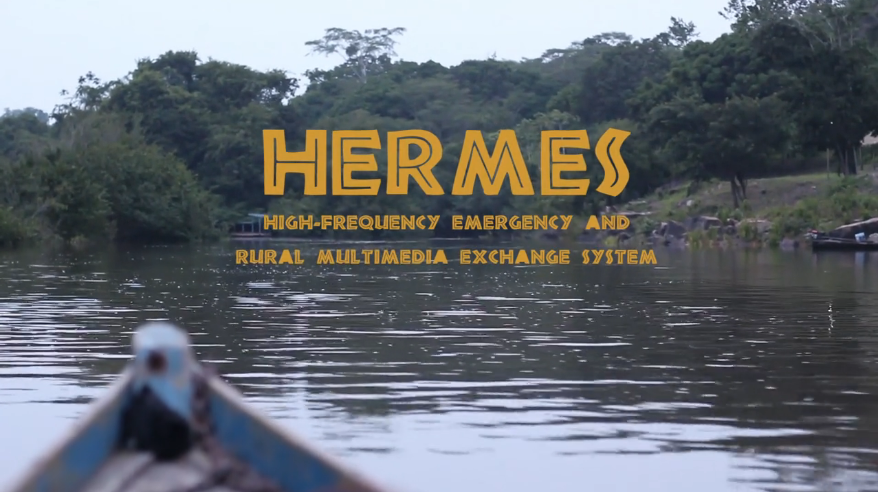
\includegraphics[width=1\textwidth]{pictures/hermes.png}
\end{figure*}

\subsection{Transceptor HERMES HF}

O painel frontal do equipamento é mostrado na figura~\ref{fig:frontview}.

A caixa do sistema HERMES inclui as seguintes entradas e saídas, mostradas na figura~\ref{fig:backview}.

\begin{enumerate}
    \item Painel traseiro - Número de Série;
    \item Painel traseiro - Conector para fio terra;
    \item Painel traseiro - Aberturas de ventilação;
    \item Painel traseiro - Conector para a antena HF (PL-259 / UHF fêmea);
     \item Painel traseiro - Fusível (10A);
     %fuse number
    \item Painel traseiro - Entrada de energia 12V DC, terminais positivo (vermelha) e negativo (preta);
    \item Painel traseiro - Conector para antena WiFi (RP-SMA fêmea);
    \item Painel traseiro - Entrada Ethernet RJ-45, para conexão em switch externo ou roteador;
    \item Painel frontal - Botão de energia (on/off);
    \item Painel frontal - 4 LED's indicadores (LED do Sistema, LED de estado da antena, LED conectado, LED TX).
\end{enumerate}

\begin{figure}[!ht]
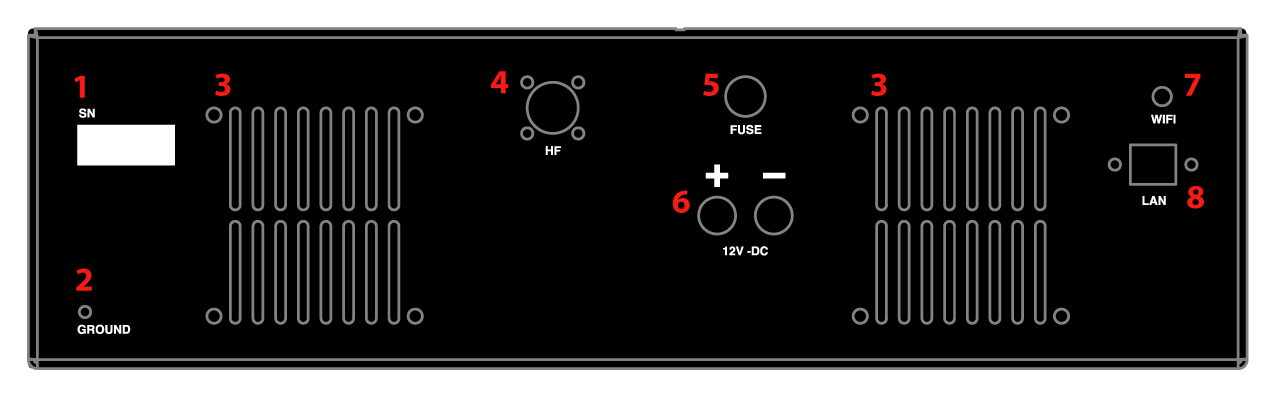
\includegraphics[width=1\textwidth]{pictures/traseiro.png}
\caption{Vista traseira da caixa do Hermes}
\label{fig:backview}
\end{figure}

\begin{figure}[!ht]
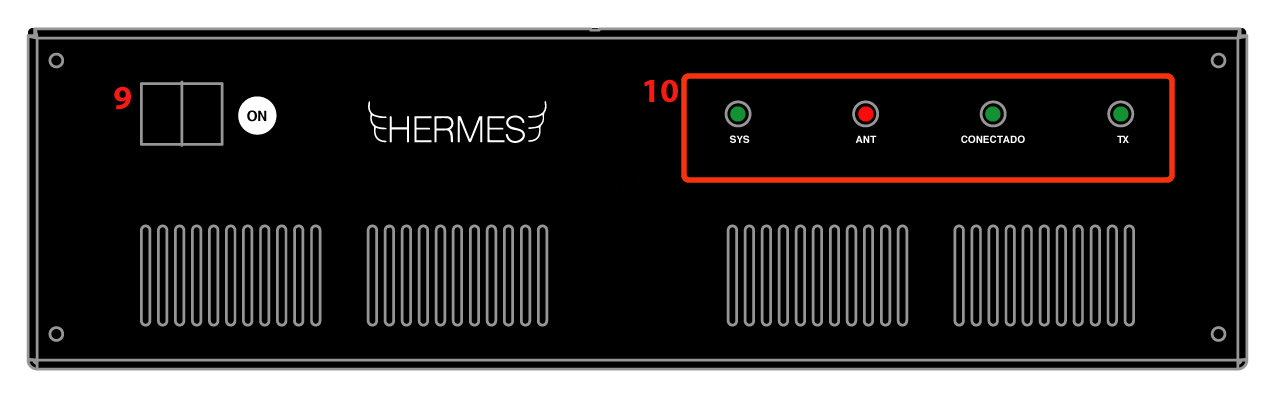
\includegraphics[width=1\textwidth]{pictures/front.png}
\caption{LEDs indicadores no painel frontal}
\label{fig:frontview}
\end{figure}
Os LEDs indicadores estão configurados para mostrar o seguinte:
\begin{itemize}
    \item SYS: LED do Sistema, pisca quando o equipamento ainda não está pronto para o uso. Esse LED normalmente pisca quando o sistema está ligando ou desligando;
    
    
    %System LED, blinks when the system is not ready to be used. SYS LED typically blinks when the equipment is turning on or when it is turning off;
    \item ANT: Verde quando a antena está funcionando corretamente, e nenhum valor alto de ROE (SWR) está detectado. Este LED fica vermelho quando um valor alto de ROE (SWR) for detectado, indicando que a proteção contra alto ROE (SWR) está ativada e o rádio não vai transmitir. Se a proteção estiver ativada, precisa ser reiniciada pela interface administrativa do rádio. Antes de reiniciar a proteção pela interface web, cheque a antena e o cabo de HF;
    
    %Green when the antenna is functioning properly, and no high SWR value is detected. ANT LED turns Red when a high SWR value is detected, meaning the high SWR protection is enabled and the radio will not transmit. SWR protection needs to be reset if active (Red), for the radio to became operational again, which can be done in the radio administrative interface. Check the RF cable and Antenna before resetting in the interface;
    \item CONECTADO: Se o LED estiver verde sólido, indica que a estação está conectada a outra estação;
    
    
     
    
    %LED on (solid Green) means that the station is connected to another station;
    \item TX: Quando o LED estiver ligado, significa que o rádio está transmitindo. Se estiver desligado, o rádio estará em modo de recepção. Se o LED CONECTADO estiver ligado e o LED TX estiver deligado o rádio está recebendo dados. Durante uma comunicação ativa com outra estação, o LED CONECTADO permanecerá verde enquanto o LED TX vai ligar e desligar.
    
    %LED on means the radio is transmitting. When this LED is off, it is in receive mode. If the CONECTADO LED is on and the TX LED is off, the station is actively receiving. During active communication with another station the CONECTADO LED will be solid Green and the TX LED will turn on and off;
\end{itemize}


\subsection{Recomendação de antena HF}

Uma antena sintonizada na operação de frequência desejada precisa estar conectada ao equipamento. Nunca ligue o equipamento antes de conectar uma antena apropriada! 

%An HF antenna tuned to the desired operating frequency must be connected to the equipment. Never turn on the equipment without first connecting to an appropriate antenna!

Existem vários tipos de antena para diferentes propósitos. Para comunicação de médio e curto alcance (até 800km), um dipolo de quarto de comprimento de onda instalado em uma configuração de V invertido é uma boa opção de custo acessível.

%There are many HF antennas, each one fitting a different purpose. For short and medium range communications (up to about 800 km), a quarter wavelength dipole installed in inverted V configuration is a good and affordable option. %could include a link to the Rhizomatica HF manual here. 

\subsection{Requisitos de Energia}

O sistema é desenhado para operar com potência entre 12V DC e 14V DC. Um sistema típico pode utilizar uma bateria de 12V DC de uma bateria conectada a um controlador de carga solar e painéis fotovoltaicos. Outra opção é utilizar uma fonte de energia de 12V ou 13.8V AC/DC. 

%The system is designed to operate with between 12V DC to 14V DC power. A typical setup would use 12V DC from a battery connected to a solar charge controller and photo-voltaic panels. Another setup option is to use a 12V or 13.8V AC/DC power supply. 

O conector vermelho na parte de trás do equipamento deve ser conectado com a saída de polaridade positiva (+) da bateria ou fonte de energia, enquanto o conector preto deve recber a polaridade negativa (-). O sistema tem uma proteção quanto à inversão de polaridade, mas deve-se ter cuidado de instalar corretamente as entradas de energia. O transceptor consome aproximadamente 2A no modo receptivo e 6A no modo transmissor.

%The red connector on the back of the transceiver should be connected to the positive (+) polarity of the battery or power supply unit, while the black connector to the negative (-) polarity. The system has polarity inversion protection, but care should be taken to proper power installation of power connections. The transceiver consumes approximately 2A in receive mode, and 6A in transmit mode. %is receive mode the same thing as standby?

\section{Interface web}

O Sitema Hermes oferece uma interface web que pode ser acessada através da rede local WiFi. Para acessar a rede Hermes pelo WiFi do seu dispositivo, utilize os seguintes dados 
%HERMES provides a web interface which can be accessed through a local WiFi network. When accessing the HERMES WiFi network, the following information applies:
\begin{itemize}
    \item Nome da Rede (ESSID): HERMES
    \item Senha: amazonia
\end{itemize}

Saiba que ao acessar a rede Hermes através de alguns dispositivos, o navegador vai abrir automaticamente a página principal do sistema Hermes, enquanto em outros é preciso acessá-la através do endereço \url{http://hermes.radio} ou \url{http://10.0.0.1} pelo navegador.
O navegador chrome / chromium é o navegador padrão para utilização da interface HERMES, para garantir uma melhor experiência faça preferência pelos navegadores informados.
%Be aware that on some mobile phones a browser will automatically open with the the main HERMES web page, while in others, to access the HERMES web interface, you must open the browser and access \url{http://ac1.hermes.radio} or \url{http://10.0.0.1}.

   \begin{figure}[H]
    \centering
    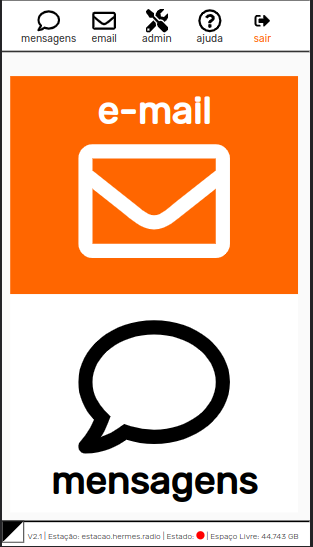
\includegraphics[width=0.5\columnwidth]{screenshots/frontend/pt_kn/landing.png}
    \caption{Hermes Home page and elements}
    \label{fig:interface}
    \end{figure}
    %TODO - Marcar imagem landing%
    
Na página principal (figura \ref{fig:interface}) você vai encontrar os seguintes recursos:

\begin{enumerate}
    \item Nome de domínio da sua estação;
    \item Menu principal;
    \item Link para a lista de mensagens públicas;
     \item Informação e links de entrar e sair (login e logout);
     \item Aba para ativação dos modos claro e escuro;
    \item Informações e estado da estação;
\end{enumerate}

A interface web permite a usuários administradores gerenciar contas de e-mail, alterar as configurações de radio (como alterar a frequência e o modo SSB) e trocar mensagens diretas entre estações. A interface também contém sua própria seção administrativa, para criação e gerenciamento de usuários e definição de seus privilégios.     
%The web interface allows admin users to manage e-mail accounts, to perform radio configurations (like setting frequency and SSB mode) and exchange direct messages between stations (BBS). The interface also contains its own administrative section, for defining and managing users and their privileges. 

É importante notar que o mesmo nome de usuário criado para a interface administrativa vai ser utilizado como endereço de e-mail para aquele usuário. Por exemplo, o usuário "amelia" na interface local vai ter o e-mail "amelia@ac2.hermes.radio". Note que o endereço de e-mail é composto pelo nome de usuário , seguido de uma "@" e o nome da estação, que corresponde ao seu nome de domínio, nesse exemplo, "ac2.hermes.radio". O nome de mínio de cada estação está escrito no cabeçalho da interface web, abaixo do logo do Hermes. 

%ga tbm nos kanindé?

%It is important to note that same user name created for the administrative interface will be used for the e-mail address assigned to that user.  For example, user "amelia" in the local interface will have the email "amelia@ac2.hermes.radio". Note that the email address is composed of the user name @ the name of the station, which corresponds to its internet domain name, in this example, "ac2.hermes.radio". Each station domain name is written in the header on the Hermes web interface. If the domain begins with "ga" then it is a Gateway station.

\subsection{Interface administrativa}
\label{admininterface}

\begin{figure}[H]
    \centering
    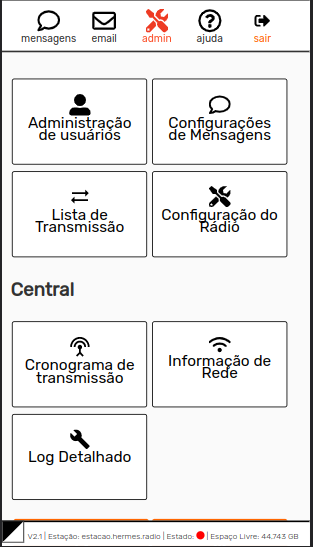
\includegraphics[width=0.5\columnwidth]{screenshots/frontend/pt_kn/admin.png}
    \caption{Interface administrativa}
    \label{fig:admin}
\end{figure}

Para acessar os recursos de administração, você precisa de uma senha de administrador. Apesar de todo mundo conseguir criar uma conta de usuário, somente administradores do sistema podem criar novos usuários administradores, ou dar poderes de administrador para outros usuários. Para fazer entrar, clique no ícone de login no topo à direita da interface web.

%To access admin features, you need an admin password. While anyone can create a user account, only a system admin can create new administrator user and give admin power to other users. To login, click on the login icon on the top right of the web interface. 

O username de login de administrador padrão é "root" e a senha é "caduceu".

%The default administrator login username is: "root" and the password is: "caduceu".

Dentro da seção de administração, um administrador vai encontrar as seguintes opções: gerenciamento de usuários, configuração de mensagens, informações da rede, estações, registros detalhados e configuração de rádio. Se a estação for uma estação central, vai haver também um menu de estação central.
%Inside the administration section, an admin user will find the following options: user management, messages administration, network information, stations, detailed log and radio configuration.

\subsubsection{Gerenciamento de Usuários} 

Permite a criação de novos usuários, atualização dos dados de usuários registrados e deletar usuários do sistema. Cada nome de usuário corresponde a uma conta de email com o mesmo nome, como no exemplo acima (ex: amelia@ac2.hermes.radio).
%Allows the creation of new users, updating data of registered users and to delete users of the system. Every username corresponds to an email account with the same name as in the example above (e.g. amelia@ac2.hermes.radio).%
    
    \begin{figure}[H]
    \centering
    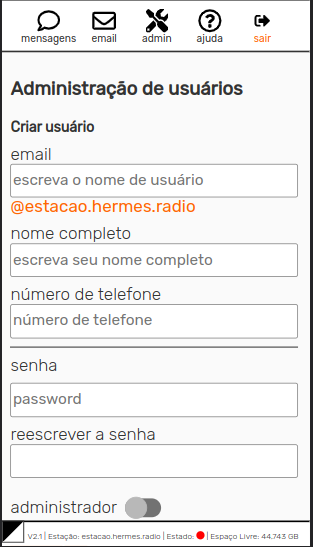
\includegraphics[width=0.5\columnwidth]{screenshots/frontend/pt_kn/createuser.png}
    \caption{Interface de criação de usuário}
    \label{fig:createuser}
    \end{figure}
    
    Administradores também podem dar poderes de administração para usuários regulares, clicando na caixa de seleção "é administrador" no final do formulário de criação de usuário.
    %Administrators can also give admin powers to regular users, by clicking on the "is admin" checkbox at the bottom of the Create User page.

\subsubsection{Configuração de Mensagens}  
\label{gui_msg_admin}

A partir desta página, um administrador pode determinar quem pode enviar mensagens públicas entre estações e quem pode anexar arquivos nessas mensagens: somente administradores, somente usuários registrados ou todo mundo. É bom pensar em restringir isso uma vez que anexar arquivos pode reduzir consideravelmente a velocidade do sistema.


%From this page, an admin can determine who will be able to attach files to public messages between stations: everyone; only registered users or only administrators. It is worth thinking this through with the users as attachments can slow the system down considerably.
   
    \begin{figure}[H]
    \centering
    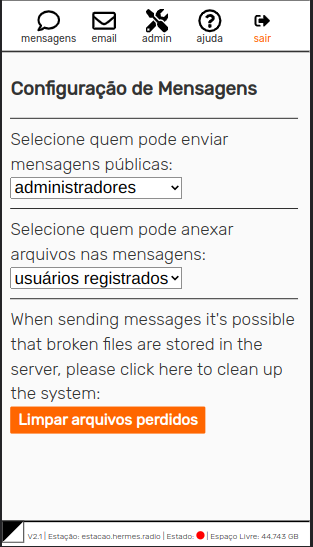
\includegraphics[width=0.5\columnwidth]{screenshots/frontend/pt_kn/messageadm.png}
    \caption{Interface de configuração de mensagens}
    \label{fig:messageadm}
   
    \end{figure}


\subsection{Lista de transmissão}
\label{gui_trans_list}

Toda troca de dados do sistema HERMES acontece através do protocolo UUCP, um sistema assíncrono, uma vez que os dados vão para uma fila antes de serem transmitidos. Os elementos da fila do UUCP são chamados de "trabalhos, cada trabalho do sistema HERMES pode ser um e-mail, uma mensagem, ou um comando especial para execução remota (por exemplo, para informar a criação de um novo usuário). Um administrador do sistema pode cancelar um trabalho antes que ele seja enviado. Administradores podem também apagar as mensagens públicas por qualquer razão, incluindo o caso quando o espaço de armazenamento do equipamento estiver atingindo o seu limite. O espaço de armazenamento disponível é mostrado no rodapé da interface. 

%All data exchange in the HERMES system is done through UUCP. Being an asynchronous protocol, all the data is first queued before being transmitted. The elements of the UUCP queue are called "jobs", and each job in the HERMES system can be an e-mail, a public message, or special remote command execution message (for example, to inform of a new e-mail user creation). A system administrator can cancel a job before it is sent. Administrators can also erase the public messages for any reason, including the case when the equipment storage space is reaching its limit. The storage space available is shown in the web interface footer.

A filas de todas estações são transmitidas periodicamente quando a estação central conecta com cada estação remota baseada nos horários de agendamento que estiverem configurados. em uma emergência, um administrador do sistema pode forçar a transmissão de mensagens entre estações, clicando no botão "forçar". Isto pode interromper a recepção de mensagens de outras estações por um tempo e deve ser evitado a não ser que seja absolutamente necessário.

%The queues of all Host stations are transmitted periodically when the Gateway station connects to each remote station based on whatever schedule has been configured. In an emergency, a system administrator can force message transmission and bypass the queue by clicking on the "transmit now" link. This could interrupt receiving messages from other stations for a while and should be avoided unless absolutely necessary.   
    \begin{figure}[H]
    \centering
    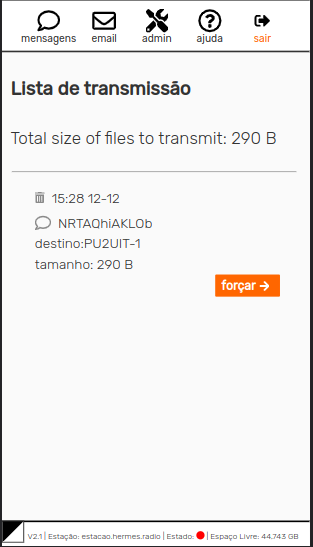
\includegraphics[width=0.5\columnwidth]{screenshots/frontend/pt_kn/transmission.png}
    \caption{Interface da lista de transmissão}
    \label{fig:transmission}
   
    \end{figure}    
    
    
\subsubsection{Configuração do Rádio}
\label{gui_radio_config}

Apresenta uma interface direta para mudar várias configurações do rádio como frequência, modo transmissão, resetar configurações de fábrica e também permite que se faça leituras dos sensores do rádio sobre a antena HF do sistema.

%Provides a direct interface to change various radio settings like frequency, transmission mode, restore factory configuration and it also allows one to view sensor readings about the HF antenna of the system. 

%we should provide more in-depth information about what the values mean, what to be careful about changing, etc.

\begin{figure}[H]
    \centering
    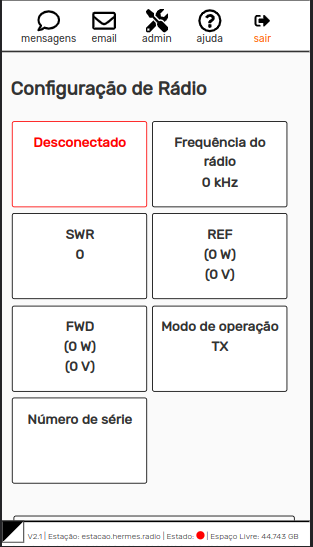
\includegraphics[width=0.5\textwidth]{screenshots/frontend/pt_kn/radioconfig.png}
    \caption{Interface de configuração do rádio}
	\vspace{-10pt}
    \label{fig:radioconf}
\end{figure}    

\begin{figure}[H]
    \centering
    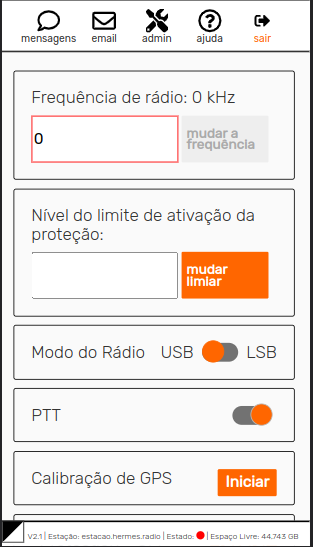
\includegraphics[width=0.5\textwidth]{screenshots/frontend/pt_kn/radioconfig2.png}
    \caption{Interface de configuração do rádio}
	\vspace{-10pt}
    \label{fig:radioconf2}
\end{figure}   

\subsubsection{Estação central} 
\label{gui_central_station}

A estação central é uma estação especial que se mantém conectada à internet. Se estiver em uma estação central, esta opção aparecerá no menu. Dela é possível criar horários de agendamento para transmissão para outras estações, que são períodos de tempo onde as transmissões vão acontecer entre todas estações conectadas à rede. Também é possível habilitar ou desabilitar os agendamentos ou alterar seus horários de funcionamento através deste menu.

%The central station is a special station that keeps connected to the internet. If you are in the central station, this option will be shown in the menu. From there is possible to create schedules for transmission to other stations, that are the time slots when the transmission will happen between all the stations connected to the network. It's possible also to enable or disable schedules or change their times from this menu.

\begin{figure}[H]
    \centering
    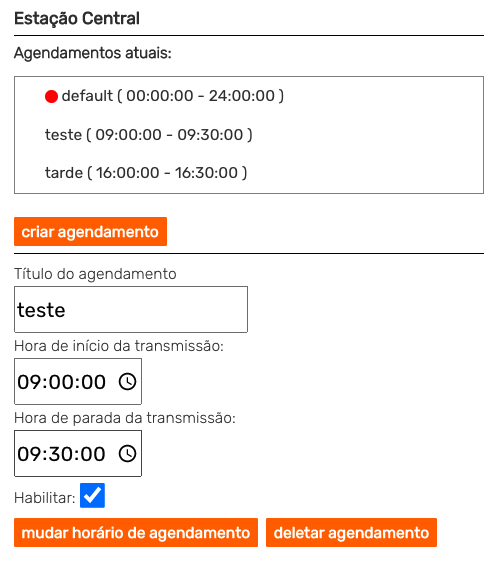
\includegraphics[width=0.5\textwidth]{screenshots/frontend/pt_kn/central.png}
    \caption{Stations interface}
	\vspace{-10pt}
    \label{fig:central}
\end{figure} 

\begin{figure}[H]
    \centering
    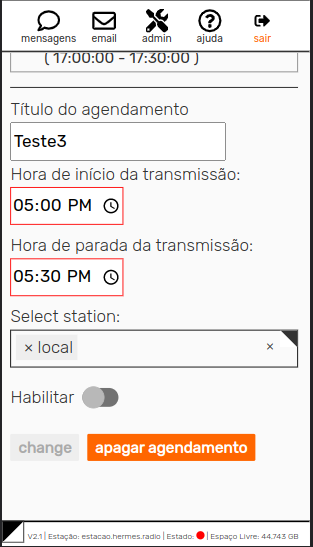
\includegraphics[width=0.5\textwidth]{screenshots/frontend/pt_kn/central2.png}
    \caption{Stations interface}
	\vspace{-10pt}
    \label{fig:central2}
\end{figure}

\subsubsection{Informações de rede} 
\label{gui_net_info}

Mostra algumas informações sobre o sistema como endereços de rede, callsign, nome do servidor etc.
%Displays some information about the system, such as network addresses, callsign, servername etc
     \begin{figure}[H]
     \vspace{-10pt}
    \centering
    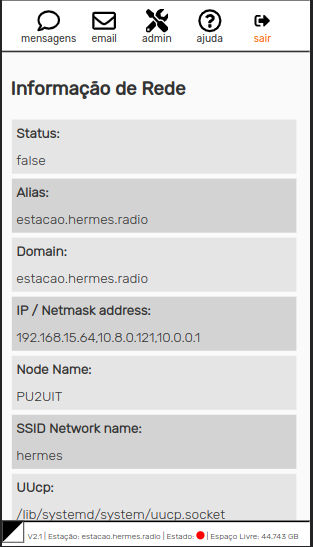
\includegraphics[width=0.5\columnwidth]{screenshots/frontend/pt_kn/networkinfo.png}
    \caption{Página de Informações de rede}
    \label{fig:netinfo}
\end{figure}
    

\subsubsection{Estações} 
\label{gui_stations}

Apresenta uma lista das estações disponíveis no sistema. 
% Se a estação for uma estação central pode-se escolher quais estações estarão habilitadas para transmitir e receber mensagens. 
%Provides a list of the available stations on the system. If the station is a gateway station, you can choose which stations will be enabled to transmit and receive messages.

\begin{figure}[H]
    \centering
    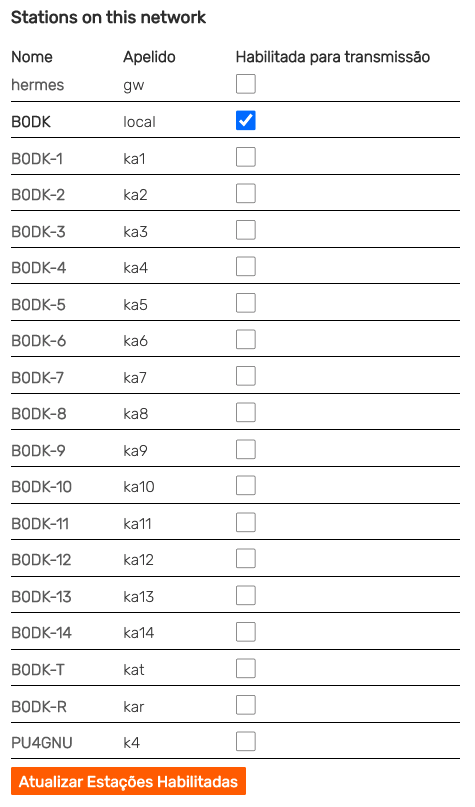
\includegraphics[width=0.4\textwidth]{screenshots/frontend/pt_kn/stations.png}
    \caption{Interface da Lista de Estações}
    \vspace{-10pt}
    \label{fig:stations}
\end{figure} 


    
\subsubsection{Registros Detalhados}
Oferece acesso aos registros dos sistema como os registros de e-mail e de UUCP, que registram cada atividade ocorrida no sistema.
%Provides access to system logs, such as email logs and UUCP logs, that register every activity on the system.
    
    \begin{figure}[H]
    \centering
    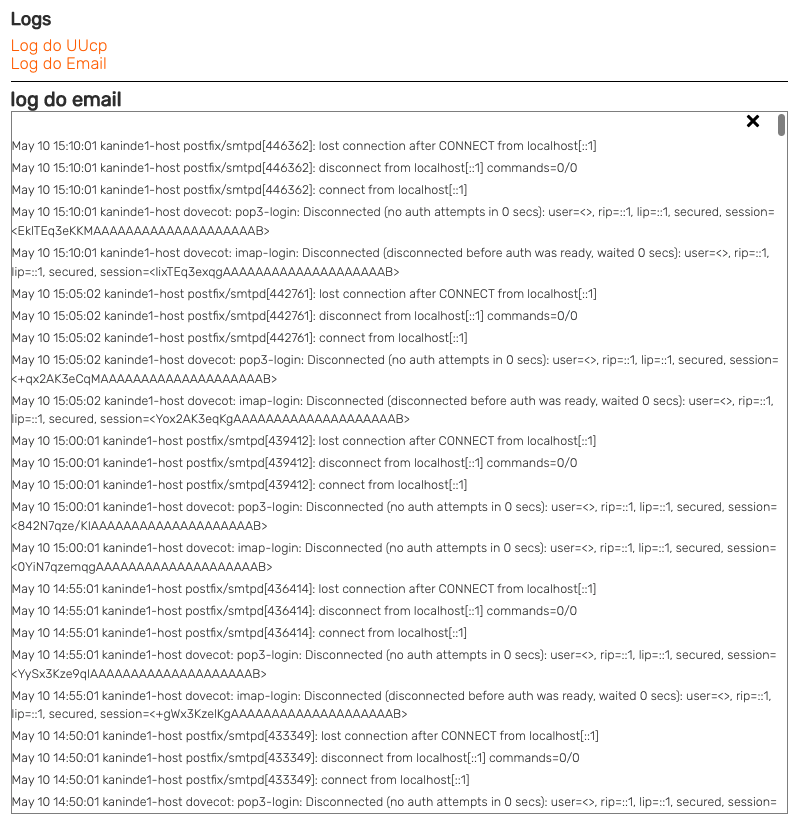
\includegraphics[width=0.5\columnwidth]{screenshots/frontend/pt_kn/logs.png}
    \caption{Página dos registros detalhados}
    \label{fig:logs}
\end{figure}



\subsection{Mensagens Públicas  (BBS)}

Mensagens diretas com suporte à criptografia e compressão de imagens podem ser enviadas entre estações. As mensagens públicas enviadas ou recebidas pode ser encontradas na aba de mensagens da interface. Um administrador do sistema pode escolher quem pode enviar mensagens públicas para outras ou para a própria estação.
%Direct messages can be sent between stations with support for cryptography and multimedia compression. Sent and received messages can be found in the Messages tab of the web interface. One Admin of the system can select who will be able to send public messages to other stations.

\subsubsection{Como escrever mensagens públicas}


\begin{figure}[H]
    \centering
    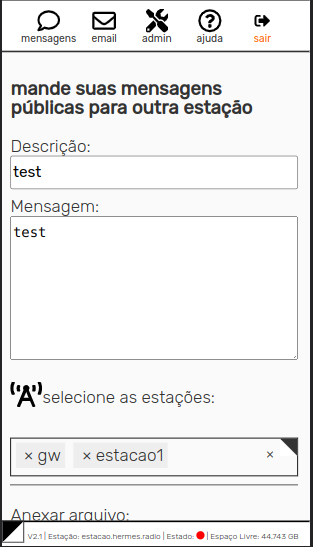
\includegraphics[width=0.5\textwidth]{screenshots/frontend/pt_kn/publicas.png}
    \caption{Interface para escrever mensagens}
    \label{fig:compose}
\end{figure}


\begin{figure}[H]
    \centering
    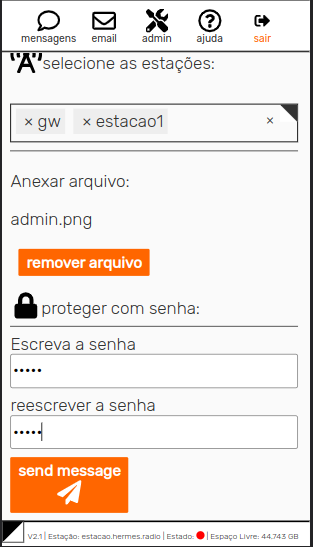
\includegraphics[width=0.5\textwidth]{screenshots/frontend/pt_kn/publicas2.png}
    \caption{Interface para escrever mensagens}
    \label{fig:compose2}
\end{figure}

Ao clicar no botão de "escrever mensagens"
% (
\includegraphics[height=0.8\baselineskip]{pictures/edit.png}) 
é possível escrever uma mensagem nova e adicionar a ela arquivos como imagens ou áudios. O ícone só irá aparecer se for permitido aos usuários compor mensagens naquela estação. Um administrador pode determinar quem pode enviar mensagens públicas entre estações e quem pode anexar arquivos a estas mensagens, alterando as permissões na seção de administração do sistema.


%By clicking on the compose (
\includegraphics[height=0.8\baselineskip]{pictures/edit.png})icon, it's possible to write a new message and to attach files such as images or audio files. The icon will only show up if it's allowed for the user to compose messages on the station. An admin can determine who can send public messages between stations and who can attach files to public messages by setting permissions in the admin tab. 

Mensagens públicas também podem ser enviadas para a sua própria estação, que é uma forma fácil de divulgar notícias dentro da sua própria comunidade. 
%Public messages can also be sent to your own station, which is an easy way to publicize news inside your own community.

Mensagens públicas também podem ser protegidas por senha, o que significa que somente aqueles que sabem a senha correta poderão ler o seu conteúdo. enquanto a descrição da mensagem (título) ainda poderá ser lido por todos. Tenha em mente que uma vez definida uma senha para uma mensagem ela não poderá ser alterada nem recuperada. 

%Public messages can also be password protected, which means that only recipients that know the password will be able to read their content, while the message description will still be readable by everyone. Have in mind that once a password for the message (has to be at least 4 characters) is defined, there is no way to recover it, nor to change it.

No link de configuração de mensagens na seção de administração do sistema, um administrador pode alterar quem pode anexar arquivos às mensagens públicas: todos com acesso à rede, somente usuários registrados ou somente administradores.

%On the message administration link in the admin section, a system administrator can change who can attach files to messages between stations: everyone with access to the network, only registered users, or only administrators. 

Devido à taxa de transmissão de dados por HF ser relativamente lenta, arquivos de anexo são limitados a 20kB. O sistema aceitará entrada de arquivos de imagens e de som de até 30MB e para outros formatos de arquivo até 2 MB, e vai tentar comprimi-las até que cheguem ao tamanho máximo de 20kB, utilizando técnicas de compressão de ponta. Obviamente, isto pode afetar a qualidade tanto de imagens como de áudios. Para outros formatos, um compressor simples será aplicado, e caso os anexos ainda tenham mais de 20kb depois disso, serão cancelados.

%Because the data throughput over HF is relatively low, file attachments are limited to 20KB. The system will accept inputs for image and sound up to 30 MB and for other files up to 2 MB, and will try to compress them to fit the maximum size of 20KB using state-of-the-art compression techniques. Obviously, this can have an effect on both image and sound file quality. For other file formats, a simple compressor will be applied, and messages with attachment size greater than 20 KB will be cancelled.%does this mean that if you try to send a file larger than 20KB it will automatically cancel, or does it mean that if the compression happens and it is unable to get under 20KB it will cancel?



\subsection{Linguagens suportadas}
\label{langs}

A interface do sistema HERMES também está disponível em inglês e espanhol, e estas versões podem ser acessadas na opção ajuda > linguagem
% aba de linguagens do menu principal.

%The HERMES interface is also available in Portuguese and Spanish, and these versions can be accessed on the Language tab of the main menu.

\begin{figure}[H]
    \centering
    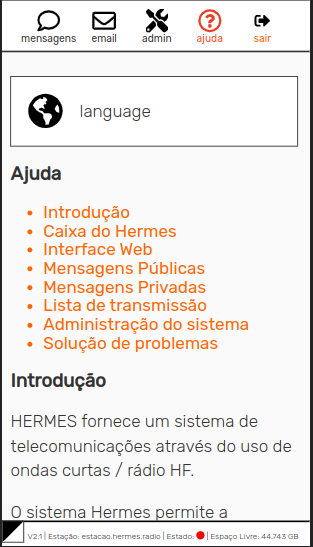
\includegraphics[width=0.5\textwidth]{screenshots/frontend/pt_kn/languages.png}
    \caption{Página de acesso às traduções}
	\vspace{-10pt}
    \label{fig:languages}
\end{figure}

\begin{figure}[H]
    \centering
    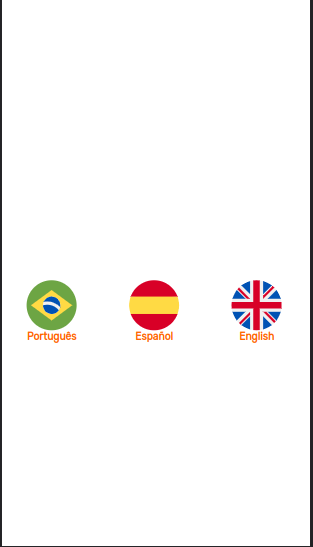
\includegraphics[width=0.5\textwidth]{screenshots/frontend/pt_kn/languages2.png}
    \caption{Página de acesso às traduções}
	\vspace{-10pt}
    \label{fig:languages2}
\end{figure}

\section{E-mail}
\label{email}

\begin{figure}[H]
    \centering
    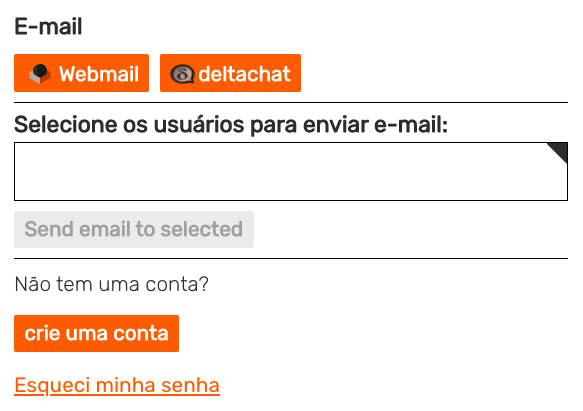
\includegraphics[width=0.5\columnwidth]{screenshots/frontend/pt_kn/email.png}
    	\caption{Pagina de acesso à interface do webmail}
	\vspace{-10pt}
    \label{fig:webmail2}
\end{figure}

Um serviço chave ofertado pelo sistema HERMES é a comunicação por e-mail. O e-mail é um protocolo de comunicação que atribui a cada usuário um endereço eletrônico no formato "nome\_de\_usuário@servidor". NO caso do sistema HERMES, a parte "nome\_de\_usuário" do e-mail corresponde ao nome de usuário definido quando um usuário é criado através da interface web, enquanto o "servidor" (também chamado de domínio) é pré-definido pelo sistema, e tipicamente terá o formato "id\_da\_comunidade.hermes.radio" . Desta forma, um e-mail HERMES poderá parecer com algo do tipo "amelia@ac1.hermes.radio". O nome de domínio da sua estação está escrito no rodapé do sistema web,
% em laranja no cabeçalho do sistema web, 
enquanto o nome do email escolhido será o nome de usuário escolhido na página de criação de usuário do sistema. 

%A key service provided by the HERMES is E-mail. The E-mail is communication protocol attributes to each e-mail bearer an address in the format "username@host". In the case of HERMES, the "username" part of the email is created by a HERMES user in the web interface, while the host (also called domain) is already set in the system, and typically has the format "community\_id.hermes.radio". So a typical HERMES emails looks like, for example, "amelia@ac4.hermes.radio". The "username" is the same username as created in the user creation page in the HERMES administration interface.

Usuários dos e-mails HERMES podem enviar e receber e-mails assim como quaisquer outros usuários de e-mail. A única restrição é que para evitar a sobrecarga do sistema com mensagens grandes, e-mails com anexos grandes serão cancelados pelo sistema, com uma mensagem de cancelamento enviada para o usuário pelo sistema.


%HERMES email users can send and receive e-mail just like any other e-mail user. The only restriction which must be considered is that in order to avoid clogging the system with large messages, emails with large attachments will be cancelled by the system, with the appropriate cancellation message sent to the user. %how large? will some compression be applied like with public messages?

Apesar de existirem vários aplicativos para envio e recebimento de e-mails, como Thunderbird ou Outlook Express, o cliente de e-mail recomendado para ser utilizado com o sistema HERMES é o Deltachat. Arquivos de instalação do Deltachat para Android, Windows, MacOs e Linux estão disponíveis para baixar pela interface. Uma outra opção é utilizar o webmail RoundCube que também é acessível pela interface web do HERMES.

%While there are many e-mail clients, like Thunderbird and Outlook Express, the recommended e-mail client to be used with HERMES is DeltaChat. DeltaChat installers are available for download through the interface for Android, Windows, MacOS and Linux. A backup option is to use RoundCube webmail which is also accessible through the HERMES web interface.

\subsection{DeltaChat}

\begin{figure}[H]
    \centering
    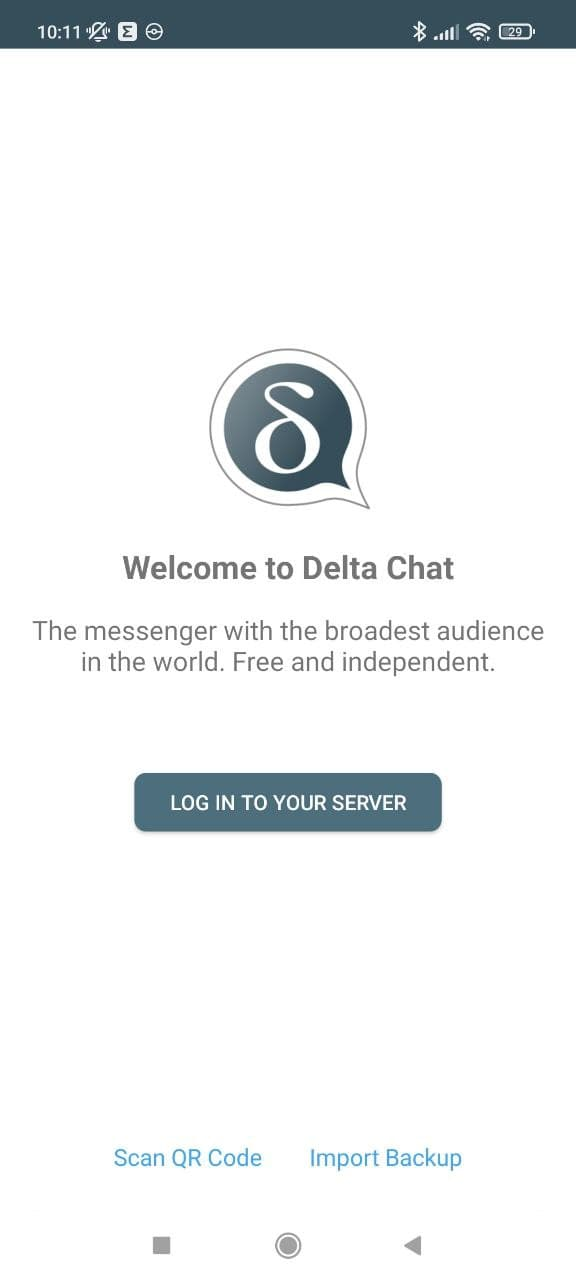
\includegraphics[width=0.3\columnwidth]{screenshots/deltachat/en/intro.jpg}
    	\caption{Instrodução do Deltachat (primeira tela)}
	\vspace{-10pt}
    \label{fig:deltachat-intro}
\end{figure}

\begin{figure}[H]
    \centering
    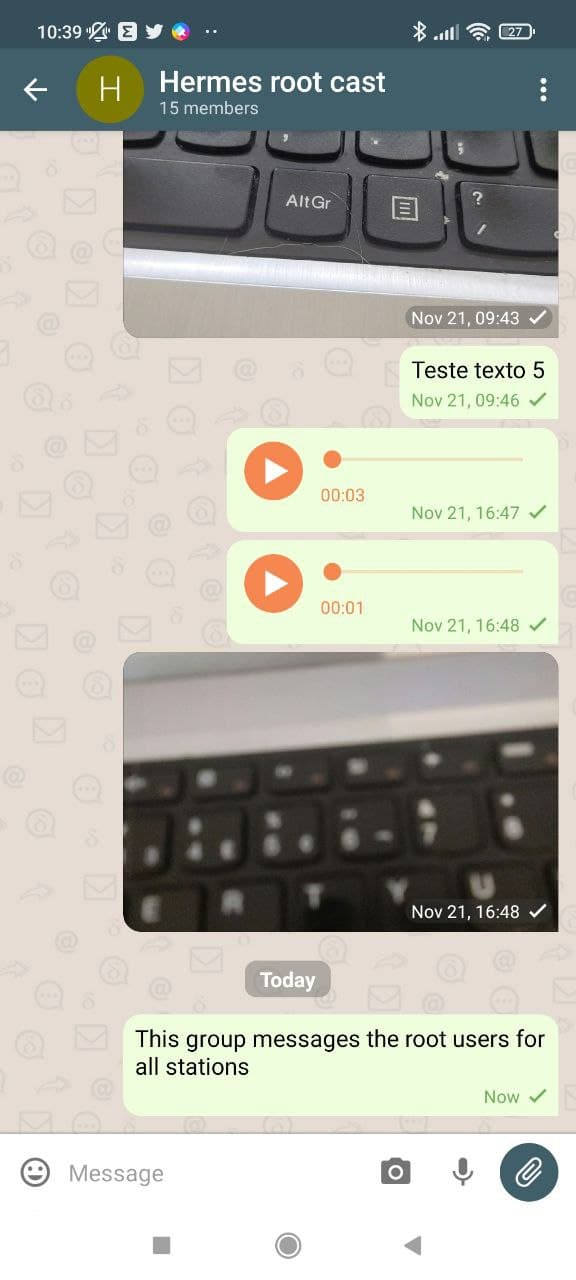
\includegraphics[width=0.3\columnwidth]{screenshots/deltachat/en/chatroom.jpg}
    	\caption{Exemplo de sala do Deltachat}
	\vspace{-10pt}
    \label{fig:deltachat-chatroom}
\end{figure}

Com o aplicativo DeltaChat, você pode utilizar o e-mail HERMES para trocar mensagens pessoais. O aplicativo funciona na maioria dos smartfones e é parecido com aplicativos comuns de troca de mensagens como com WhatsApp, Telegram ou Signa. Tenha em mente que devido ao agendamento dos horários de transmissão, as mensagens podem levar um tempo para chegar, dependendo da quantidade de mensagens na fila de transmissão e a duração das janelas de transmissão entre estações. 

%With the DeltaChat application, you can use HERMES email to carry out personal communications for exchanging messages. This app works on most common smartphones and feels like a common messaging application like Telegram, WhatsApp or Signal. Keep in mind that due to the message transmission schedule, messages may take a while to arrive, depending on the amount of messages in the queue and the transmission window length.

\subsubsection{Instalação}

O Deltachat está disponível de forma gratuita na maioria das lojas de aplicativos dos sistemas operacionais dos celulares e repositórios de arquivos. Como o Hermes é programado para funcionar em locais com pouca ou nenhuma conectividade à internet, é possível baixá-lo pela interface web do sistema, selecionando o pacote de acordo com o sistema operacional do seu dispositivo. O sistema HERMES oferece arquivos de instalação para dispositivos móveis ou computadores pessoais como Android, GNU/Linux, Windows e MacOSx. Se você estiver lendo este arquivo utilizando uma rede do sistema HERMES, os arquivos de instalação podem ser encontrados aqui: \href{ http://10.0.0.1/dowloads/deltachat.apk}{Android},  \href{ http://10.0.0.1/dowloads/deltachat.exe}{Windows},  \href{ http://10.0.0.1/dowloads/deltachat.deb}{Debian} and \href{http://10.0.0.1/dowloads/deltachat.dmg}{Mac OS}

%DeltaChat is available in most common app stores and repositories. As HERMES is designed for places with low or no connectivity, it is possible to download it through the HERMES web interface, selecting one of the packages provided according to your device operational system. HERMES provides installation files for mobile or computer systems such as Android, GNU/Linux, Windows and MacOSX. The installer files can be accessed here if you're reading this using a HERMES system network: \href{ http://10.0.0.1/dowloads/deltachat.apk}{Android},  \href{ http://10.0.0.1/dowloads/deltachat.exe}{Windows},  \href{ http://10.0.0.1/dowloads/deltachat.deb}{Debian} and \href{http://10.0.0.1/dowloads/deltachat.dmg}{Mac OS}

% FEITO qual endpoint do frontend?

\subsubsection{Configuração}

O sistema HERMES inclui um sistema de compressão adequado para que mensagens multimeios como imagens ou áudio sejam enviadas pela rede HF. Para permitir que esses sistema funcione corretamente, o usuário deve desabilitar a opção de criptografia ponto-a-ponto na configuração do DeltaChat, ou então não será possível enviar imagens e áudios.

%The HERMES system includes a compression system suitable for multimedia messages like images or audio being sent over HF.  End-to-end encryption should be disabled in order to allow the server-based image and audio compression to work properly, otherwise image and audio exchange will not be possible.

Os passos para encontrar este recurso no Deltachat são: Menu de Hambúrger (
\includegraphics[height=0.78\baselineskip]{pictures/burger.png}) -> Configurações -> Avançado -> Autocrypt. Desligar a opção preferir criptografia de ponta-a-ponta, como monstrado na Figura~\ref{fig:deltachat-adv_p2pe}.

%The steps to find this feature in Deltachat are: Burger Menu (
\includegraphics[height=0.78\baselineskip]{pictures/burger.png}) -> Settings -> Advanced -> Autocrypt, turn off: Prefer End-To-End Encryption) as shown in Figure~\ref{fig:deltachat-adv_p2pe}.

\begin{figure}[H]
    \centering
    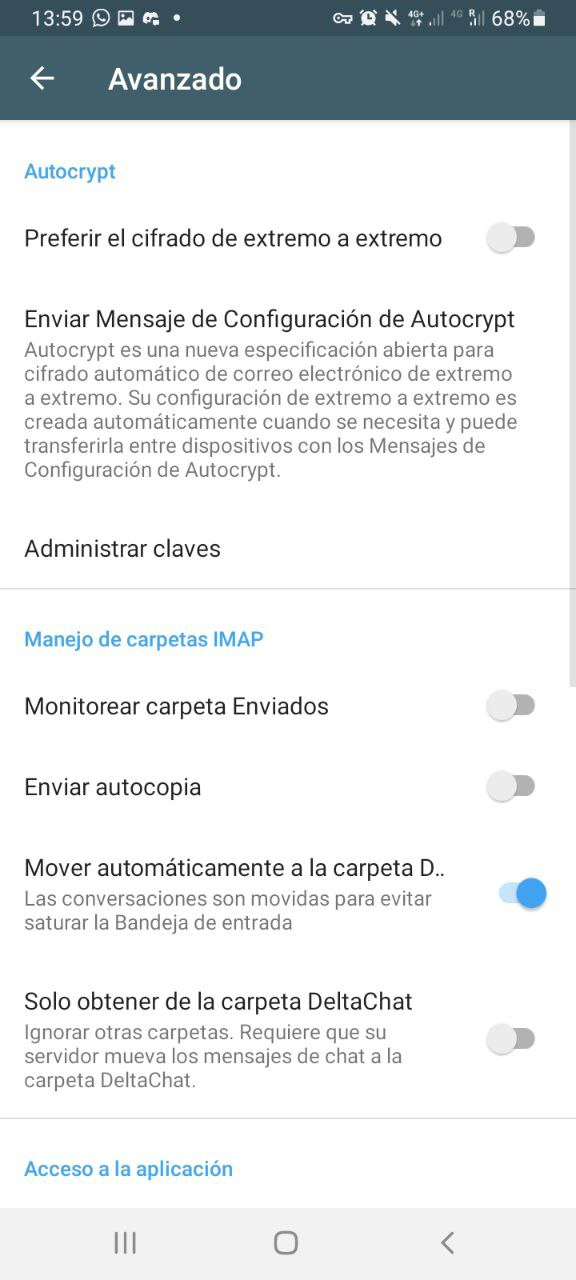
\includegraphics[width=0.3\columnwidth]{screenshots/deltachat/es/adv_p2pe_es.jpeg}
    	\caption{Configurações avançadas do DeltaChat}
	\vspace{-10pt}
    \label{fig:deltachat-adv_p2pe}
\end{figure}

Deltachat, por padrão, marca as mensagens e mostra somente mensagens "e-mail" que foram enviadas por outros aplicativos DeltaChat. Para receber e-mails escritos por quaisquer clientes de e-mail, habilite a opção "mostrar todos e-mails".

%Deltachat, by default, tags its emails and show only the "known" messages (emails) that was sent by another Deltachat application. In order to be able to interact with e-mails from any e-mail client software, enable the option "show all emails".

Os passos para encontrar este recurso são: Menú de Hambúrguer (
\includegraphics[height=0.78\baselineskip]{pictures/burger.png}) -> Configurações -> Conversas e Mídia -> Mostrar e-mails clássicos -> Todos. Como mostrado na figura~\ref{fig:deltachat-allemails} 

%The steps to find this feature in Deltachat are:  Burger Menu (
\includegraphics[height=0.78\baselineskip]{pictures/burger.png}) -> Settings -> Chats and Media -> Show Classic E-Mails -> All. As shown in Figure~\ref{fig:deltachat-allemails}

\begin{figure}[H]
    \centering
    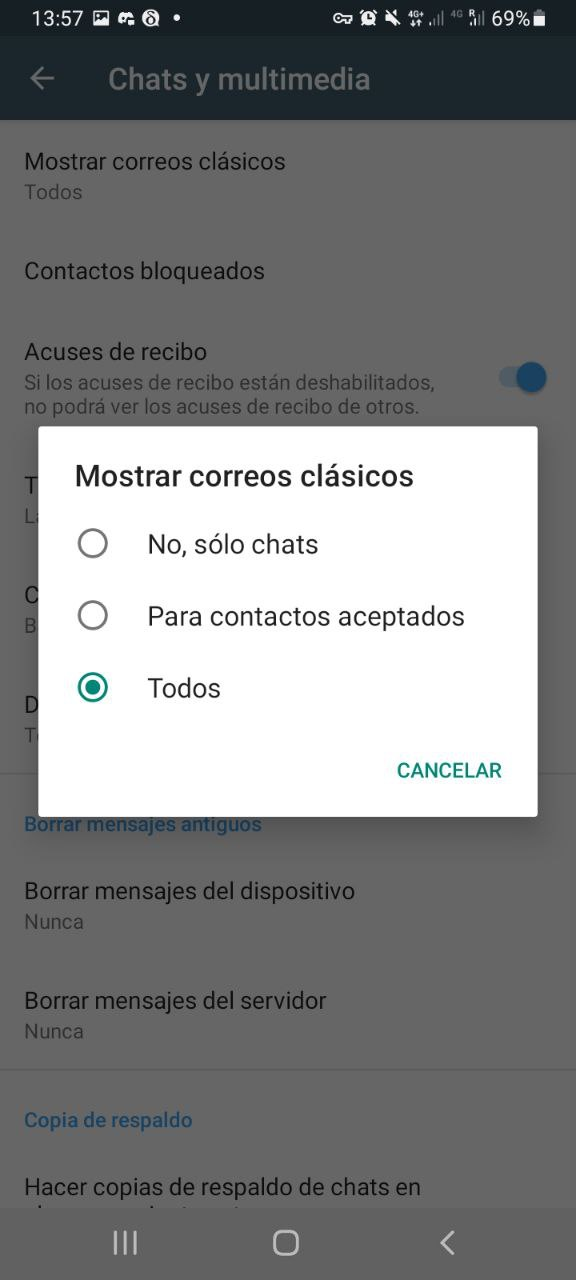
\includegraphics[width=0.3\columnwidth]{screenshots/deltachat/es/allemails_es.jpeg}
    	\caption{Configurando o DeltaChat para mostrar todos e-mails}
	\vspace{-10pt}
    \label{fig:deltachat-allemails}
\end{figure}

\subsubsection{Uso}
Para configurar o Deltachat, primeiro é necessária a criação de uma conta de e-mail, como descrito na seção~\ref{admininterface}. Para acessar uma conta de e-mail, somente os campos de endereço de e-mail e senha devem ser preenchidos, como mostrado na Figura~\ref{fig:deltachat-login}. O usuário e senha será o mesmo utilizado para criar um login para o sistema HERMES e para utilização do webmail RoundCube. 


%In order to configure DeltaChat, first an e-mail account should be created, as described in section~\ref{admininterface}. In order to login to an e-mail account, only the e-mail address and password fields should be filled, as shown in Figure~\ref{fig:deltachat-login}. The user and password will be the same as those created when first creating a login on HERMES and for use with the RoundCube webmail.

\begin{figure}[H]
    \centering
    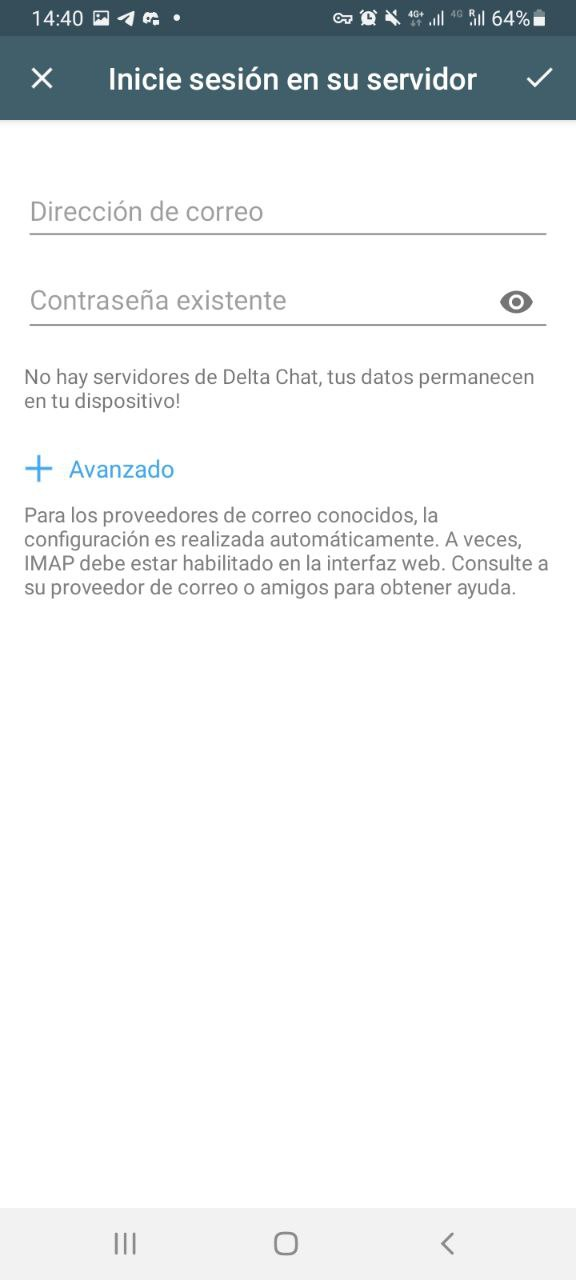
\includegraphics[width=0.3\columnwidth]{screenshots/deltachat/es/login_es.jpeg}
    	\caption{Exemplo de Login do Deltachat}
	\vspace{-10pt}
    \label{fig:deltachat-login}
\end{figure}

\subsection{Outros clientes de e-mail}

Outros clientes de e-mail também podem ser utilizados. Nós não podemos cobrir todos os casos, mas o sistema HERMES utiliza serviços padrão como IMAP para sincronizar pastas de e-mail e SMTP para enviar as mensagens. Informações mais específicas sobre as portas podem ser encontradas no apêncide: \ref{apx_net_email}

%Other email clients can also be used. We can't cover all cases, but the HERMES system uses default services like IMAP to synchronize email folders and SMTP to send the messages. Specific technical information about the ports can be found in the appendix: \ref{apx_net_email}

\section{Resolução de problemas}

A interface web do HERMES indicará quando algo estiver errado com o sistema. Quando um círculo vermelho aparecer na barra de rodapé (figura \ref{fig:status}, ele se tornará interativo e quando clicado, mostrará a lista dos serviços que estão com algum problema.

%The HERMES web interface indicates when something is wrong with the system. When a red dot appears in the footer bar (figure \ref{fig:status}), it becomes interactive, and when clicked, it lists the names of the services that are experiencing a problem.

\begin{figure}[H]
    \centering
    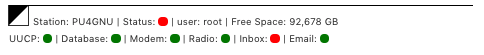
\includegraphics[width=0.8\columnwidth]{screenshots/frontend/en/status.png}
    	\caption{Círculo vermelho na interface pode ser clicado para mostras se algum serviço estiver com problemas}
    \label{fig:status}
\end{figure}

Em caso de problema com a antena, um led vermelho (ANT) se acenderá na caixa do servidor HERMES (não na interface web). Neste caso, cheque a posição e a integridade da antena, dos conectores RF, cabos coaxiais e do transmissor. Depois de checado, é necessário restaurar a proteção da antena pela interface web para que o transmissor volte a funcionar.

%In case of problems with the antenna, a red led in the antenna (ANT) position will light up on the HERMES box (not the web interface). In this case, check the correct position of the power supply wires and check the position and integrity of the antenna, RF connectors, coaxial cable, and the transmitter.

Se as mensagens na lista de transmissão não estiverem sendo transmitidas durante o período esperado, cheque se nenhuma configuração do rádio foi alterada na seção de configuração de rádio no menu de administração. Ali você poderá restaurar as configurações de fábrica, se este for o caso. Se este não for o caso, é possível que as outras estações ou a estação central esteja desligada.

%If the messages in the transmission list are not being transmitted at the allotted time, check that the radio settings have not been changed by going to the Admin tab. If that is not the case, it's possible that the other stations are offline.
%To remedy you could restore the factory default settings.



\pagebreak
\appendix{Informações Técnicas}
\label{techinfo}
\section{Apêndice - informações técnicas}
\subsection{Informações de Rede}
\label{apx_net_info}

Cada estação HERMES fornece um ponto de acesso WiFi. A configuração é:
%Each HERMES system provides a WiFi access point. The configuration is:

\begin{itemize}
\item Nome da rede WiFi: \texttt{HERMES}
\item Senha da rede WiFi: \texttt{amazonia}
\end{itemize}

O endereço IP de cada estação (na rede sem fio) é \textbf{10.0.0.1} e a conexão de rede vai conectar como um cliente dhcp a uma rede já existente.

%The IP of the HERMES station (in the wireless interface) is \textbf{10.0.0.1} and the ethernet connection will connect as a dhcp client to an already existing network. 

%\item Server address: \url{hermes.radio} (IP \url{10.0.0.1})
\subsection{Serviços de rede} 
\label{apx_net_services}

\subsubsection{Serviços de E-mail}
\label{apx_net_email}

A configuração dos e-mails é a seguinte:
%The e-mail settings are the following:

\begin{itemize}
    \item Endereço do servidor: \url{hermes} (IP \url{10.0.0.1})
    %\item Server address: \url{hermes} (IP \url{10.0.0.1})
    \item SMTP (Simple Mail Transfer Protocol): porta \texttt{25}
    \item SMTPS (Secure Simple Mail Transfer Protocol): porta \texttt{465}, com suporte para SSL  
    (utilizado para o Deltachat, os certificados são válidos até 2031)
    \item IMAP (Internet Message Access Protocol): porta \texttt{143}
    \item URL para acesso ao Webmail: \url{http://hermes/mail} or \url{http://10.0.0.1/mail}
\end{itemize}

Estas configurações não serão necessárias para a maioria dos usuários do Deltachat, já que ele identifica esses dados apenas ao escrever seu endereço de e-mail no formulário de login.

%These settings should not be needed by most users as DeltaChat automatically identifies all the settings by entering just the e-mail address and password at the login prompt.

\subsubsection{Serviços Web}
\label{apx_net_web}

A interface web HERMES roda na porta 80 para http e tem as seguintes capacidades:
%The HERMES web interface runs on port 80 on http, and provides these capabilities:
\begin{itemize}
    \item Mensagens públicas BBS P2P (sobre UUCP);
    %\item BBS P2P public messaging capability (over UUCP);

    \item Administração de e-mails de usuários;
    \item Gerenciamento da fila do UUCP;
    \item Ferramentas de gerenciamento do transceptor de rádio HF;
    \item Permissões customizadas por tipo de usuário para o envio de mensagens com arquivos multimídia;
    \item Pagina para tarefas de serviço do rádio (como gerador de tom de teste e controle de PTT);
    \item Página com informações da rede (Para casos onde o sistema HERMES se conectar com redes IP maiores);
    \item Download de arquivos executáveis do cliente do DeltaChat para Android, MacOS, Windows e Linux.
\end{itemize}

\subsection{Outros serviços de rede }
\label{apx_other_net}


\begin{itemize}
    \item SSH Secure Shell - Para uso especial administrativo: porta 22\newline
        \hfill usuário: "hermes", senha: hermes\newline
        \hfill usuário: "root" senha: "caduceu"
    \item VPN -  Virtual Private Network client pronta para acesso remoto
    %\item MQTT (Mosquitto server for network sensors integration's)
    \item ISPCONFIG interface web administrativa \newline
        \hfill porta 8080 / credenciais: "admin" "caduceu"
    \item mariaDB, o servidor de banco de dados para guardar mensagens e usuários na api da estação (station-api) e ISPconfig
    \item Serviços de e-mail com transportes conectados ao uucp
    \newline
        \hfill Postfix, dovecot, spamassin, postgrey, amavis, clamav (hold) e ISPconfig como gereciadores 
    \item iwatch: lida com a pasta inbox de HMP (mensagens públicas Hermes) e dispara o rolo de compresão UUCP
    \item hostapd: determina a interface sem fio para o modo do ponto de acesso
    \item dnsmasq: provém o nome de domínio e os apelidos 
    \item uucp: acessível pela rede com as credenciais usuário/senha%is this missing some info about user/password?
    \item VNC: Virtual X ambiente de monitoramento de sessão virtual do VARA
        \hfill porta: \texttt{5901} (Ex. na rede local WiFi: vncviewer 10.0.0.1:5901) 
        \hfill usuário: "hermes", senha: "hermes"
\end{itemize}

\section{Informação adicional}
\label{apx_adit_info}
    O sistema principal roda GNU/Linux Debian 

    The main system runs Debian GNU/Linux versão Bullseye e tentamos seguir suas linhas guia. 

\subsection{Password Cheat Sheet}
\label{passwords}

% melhor duas tabelas? Uma para o Web, outra para WiFi?
% acho redundante, já tem as senhas nos serviços também
% isso é para ser um folheto separado
% para ser impresso várias vezes
% no manual, vamos colocar numa página sozinha, ao final
% (ou no começo...)
% junto com talvez outras informações básicas de como ligar e desligar a parada talvez
% ok, entao seria separado tipo um quick guide
% talvez seja melhor separar mesmo de arquivo e limpar as senhas daqui todas - pode ser, isso vai pro github

\begin{table}[h]

\centering
\begin{tabular}{|l|l|l|}
\hline
Descrição & Usuário & Senha  \\ \hline
Interface Web & root  & caduceu \\  \hline
Rede WiFi & hermes & amazonia \\ \hline
\end{tabular}
\end{table}

\subsection{Testes de Campo}
\label{apx_field_trials}

Os protótipos do sistema HERMES foram testados em uma configuração com estações instaladas em três cidades: Brasília/DF, Belo Horizonte/MG e Hortolândia/SP. A maioria dos testes aconteceram entre Brasília e Belo Horizonte e Belo Horizonte e Hortolândia. A linha reta entre Brasília e Belo Horizonte é de 620km e entre Belo Horizonte e Hortolândia de 470km. Todas estações estavam equipadas com uma antena de dipolo simples instalada como V invertido, sintonizadas na banda de 40m de rádio amador.

    %HERMES system prototypes were tested on a test bed with stations installed in three cities: Brasília/DF, Belo Horizonte/MG and Hortolândia/SP. Most of the tests happened between Brasília and Belo Horizonte, and Belo Horizonte and Hortolândia. The straight line distance between Brasília and Belo Horizonte is 620 km, while Belo Horizonte and Hortolândia straight line distance is 470 km. All the stations are equipped with simple dipole installed as inverted V, tuned to the 40m amateur radio band.

Nos nossos testes internos, o modem atingiu mais que 1000bps em condições médias de propagação (0Db do receptor SNR). Uma mensagem de 10kb, que é o tamanho típico de um e-mail com uma imagem leva em torno de 4 minutos para ser transmitido. Em condições ruins de propagação, este tempo pode chegar até 10 minutos.

    %In our internal tests, between Belo Horizonte and Hortolândia, the modem reached more th  an 1000 bps in an average propagation condition (0db of SNR in the receiver). A 10Kb message, which is the typical size of an email with a picture takes about 4 minutes to be exchanged. In poor propagation conditions, this time can go up to 10 minutes. 

O modem adaptativo começa a comunicação a velocidades muito baixas, mas se a propagação estiver boa, ele automaticamente se prepara para aumentar a velocidade, por outro lado, se a propagação se deteriorar, o modem reduz a velocidade aumentando a robustez do sinal. 
    
    
    %The adaptive modem starts the communication with slower speeds, but if propagation is good, it gears up and automatically and increases the speed, and on the other hand, if propagation deteriorates, the modem reduces the speed, increasing the signal robustness.

\subsection{Código Fonte}
\label{apx_src}

O código fonte está disponível dentro das pastas /home/hermes/install com as últimas versões baixadas pelo Git antes da implementação e também está disponível online em: 

    %Source code is available inside the folders /home/hermes/install with the latest git versions before the deployment and is also available online at:

\begin{itemize}
    \item Interface Web Front-end, escrita utilizando o framework Angular: \url{https://github.com/Rhizomatica/hermes-gui};
    \item Interface Web Back-end, escrita em PHP: \url{https://github.com/Rhizomatica/hermes-api}; 
    \item Esquema e descriçoes do transceptor HF: \url{https://github.com/DigitalHERMES/rhizo-transceiver};    
    % TODO - Verificar repositorio
    \item Firmware e ferramentas para usuários do transceptor HF, escritas em C:
    \url{https://github.com/Rhizomatica/hermes-net};
    \item Software de gerenciamento de rede para integração entre UUCP e o modem HF (VARA ou Ardop), escrita em C:
    \url{https://github.com/DigitalHERMES/rhizo-uuardop}
    % TODO - Verificar repositorio
\end{itemize}


\section{Licenciamento}
\label{apx_license}
Todos códigos fonte do projeto são licenciados sob a versão 3 ou acima da licença GPL, a não ser que esteja explicitamente declarado no repositório.

    %All the project's source code is licensed under the GPL version 3 or any greater version, unless stated differently in the repository.

\subsection{GNU General Public License Version 3}

    High-Frequency Emergency and Rural Multimedia Exchange System (HERMES).

    Copyright (C) 2021-2022 Rhizomatica.
\newline

Este programa é um software livre: você pode redistribui-lo e/ou modificá-lo sob os termos da licença Pública GNU (GNU General Public License), como publicados pela Free Software foundation, sob a versão 3 da licença ou qualquer versão posterior (a sua escolha)

Este programa é distribuído com a esperança que seja útil, mas SEM QUALQUER GARANTIA; sem mesmo garantia implícita de COMERCIALIZAÇÃO OU SERVENTIA PARA DETERMINADO PROPÓSITO. Veja a licença pública GNU para mais detalhes. 

    %This program is free software: you can redistribute it and/or modify it under the terms of the GNU General Public License as published by the Free Software Foundation, either version 3 of the License, or (at your option) any later version.

    %This program is distributed in the hope that it will be useful, but WITHOUT ANY WARRANTY; without even the implied warranty of MERCHANTABILITY or FITNESS FOR A PARTICULAR PURPOSE.  See the GNU General Public License for more details.

Você deve ter recebido uma cópia da GNU Public License junto com este manual, se não, cheque no endereço \url{https://www.gnu.org/licenses/}

  
    
\end{document}    
